\documentclass[15pt]{beamer}
\usepackage{graphicx} % Required for inserting images
\usepackage{tikz}%for figures
\usepackage{adjustbox}
\usepackage{subfig}
\usepackage{pgfplots}\pgfplotsset{compat=1.9}
\usepackage{pgfplots}
\usepackage{amsmath}
\usepackage{amsthm} %theorems
\usepackage{amsfonts}
\usepackage{amssymb} %lesssim, etc
\usepackage{algorithm}
\usepackage[noend]{algpseudocode}
\usepackage{natbib}
\usepackage{bbm}

\usepackage{bbm}
\usepackage{xcolor}
\usepackage{hyperref}[] % hyperlink
\hypersetup{
colorlinks = true,
linkcolor = blue, %Colour of internal links
filecolor = magenta,
urlcolor = blue, %Colour for external hyperlinks
citecolor = blue, %Colour of citations
pdfpagemode=UseOutlines
}

\newcommand{\jongmin}[1]{
{ \color{blue} Jongmin: #1}
}

\newcommand\numberthis{\addtocounter{equation}{1}\tag{\theequation}}
\newtheorem{thm}{Theorem}[section]
\newtheorem{prop}[thm]{Proposition}
\newtheorem{lem}[thm]{Lemma}
\newtheorem{cor}[thm]{Corollary}


%%
%% If some other type is need, say conjectures, then it is constructed
%% by editing and uncommenting the following.
%%
\theoremstyle{definition}
\newtheorem{conj}{Conjecture}
\newtheorem{alg}{Algorithm} 
%Information to be included in the title page:
\title{Exact spike train inference via $\ell_0$ optimization}


\begin{document}

\begin{frame}
	\large
	Exact spike train inference via $\ell_0$ optimization
	\small
	\begin{itemize}
		\item Annals of Applied Statistics (2018)
		\item Written by Sean Jewell and Daniela Witten (University of Washington)
	\end{itemize}
	presenter: Jongmin Mun 
	
\end{frame}


\begin{frame}
	\tableofcontents
\end{frame}

\section{Why analyze spike trains?}
\begin{frame}

	\begin{itemize}
\item Neural spike train
\item Why do we analyze them
		\end{itemize}
\end{frame}

\begin{frame}{Spike train inference}
	\begin{figure}
		\centering
		\begin{minipage}{0.48\textwidth}
			\centering
			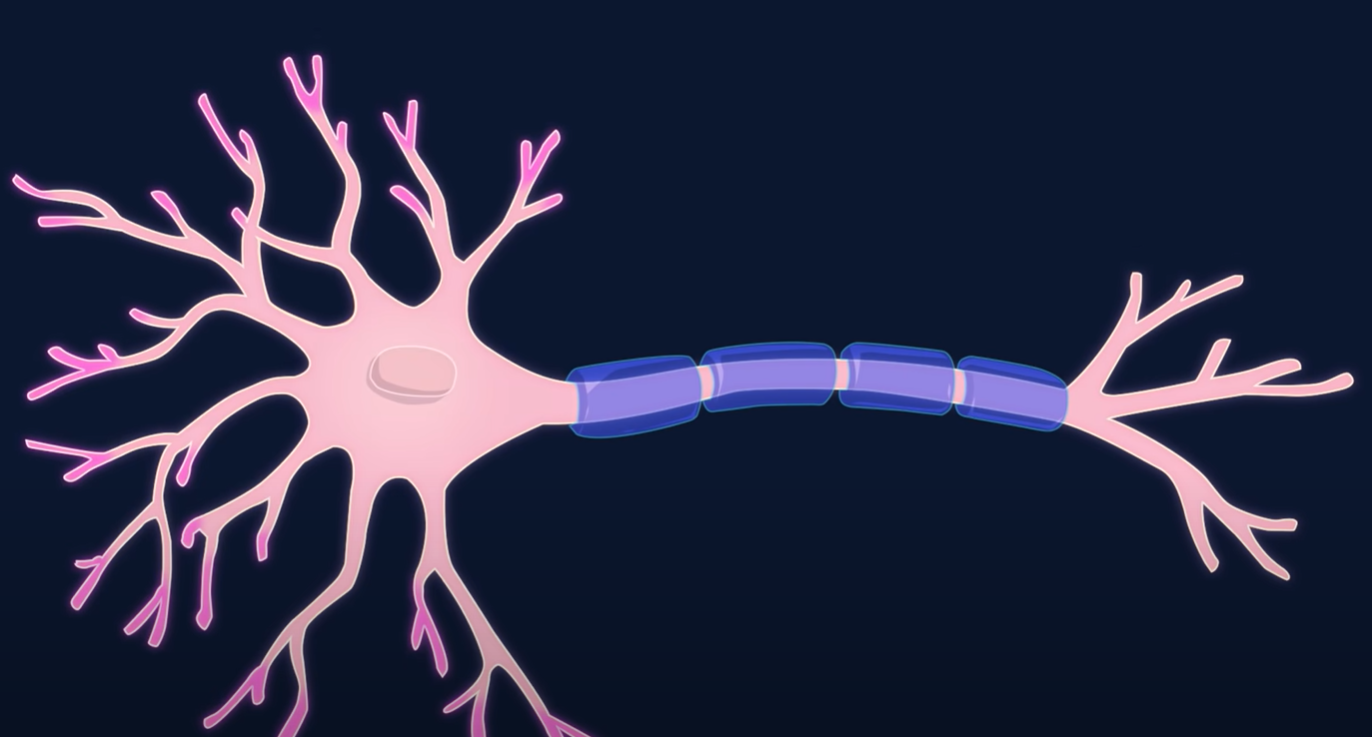
\includegraphics[width=\linewidth]{neuron}
			\label{fig:neuron}
		\end{minipage}\hfill
		\begin{minipage}{0.48\textwidth}
			\centering
			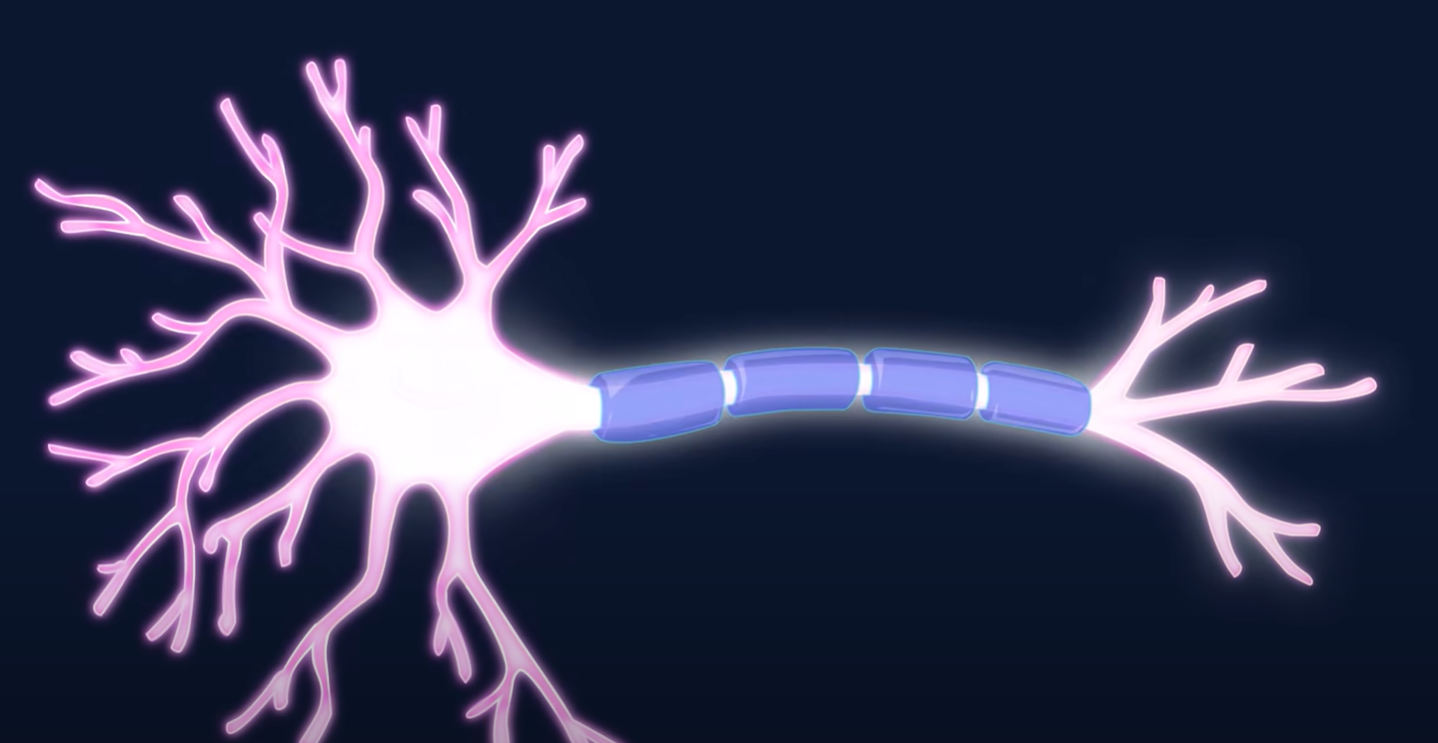
\includegraphics[width=\linewidth]{neuron_fire}
			\label{fig:neuron_fire}
		\end{minipage}
	\end{figure}
	\vskip -1cm
	\begin{figure}
	\centering
	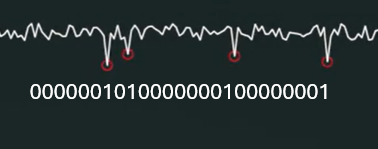
\includegraphics[width=0.4\linewidth]{binary_train}
\end{figure}
	\begin{itemize}
\item Brain operates through electrical events known as \emph{action potentials}
\item Information is primarily encoded as sequences of these action potentials: binary patterns (01010...) known as \emph{spike trains}
\item \emph{Spike train inference}: recovering these spike sequences from recorded neural electrical signals
	\end{itemize}

\end{frame}

\begin{frame}{Connection to ML}
	\begin{figure}
		\centering
		\begin{minipage}{0.48\textwidth}
			\centering
			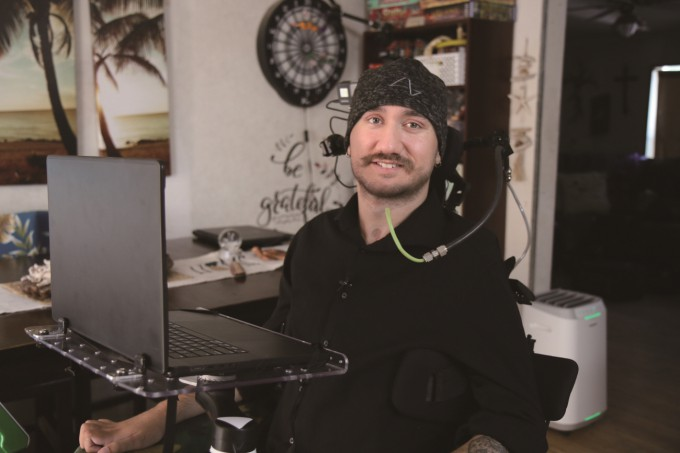
\includegraphics[width=\linewidth]{neuralink}
			\label{fig:neuron}
		\end{minipage}\hfill
		\begin{minipage}{0.48\textwidth}
			\centering
			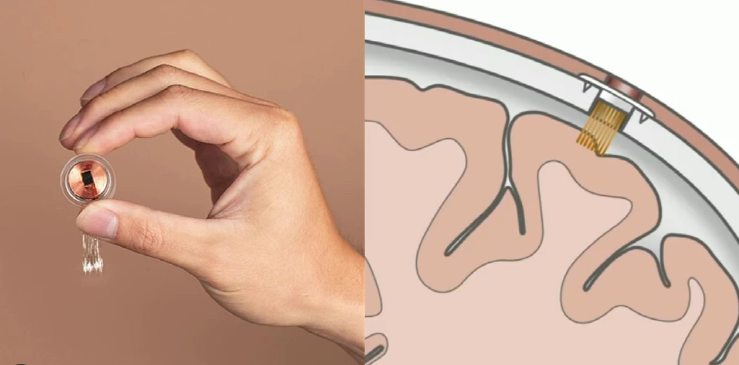
\includegraphics[width=\linewidth]{neuralink_prod}
			\label{fig:neuron_fire}
		\end{minipage}
	\end{figure}
	\begin{itemize}
\item  Spike train inference  empowers machine learning tasks such as  both \emph{brain decoding} (inferring thoughts from neural activity) and \emph{brain encoding} (translating intent into neural signals for action) 
	\end{itemize}
	
\end{frame}

\begin{frame}{Electrodes}
	\begin{figure}
		\centering
		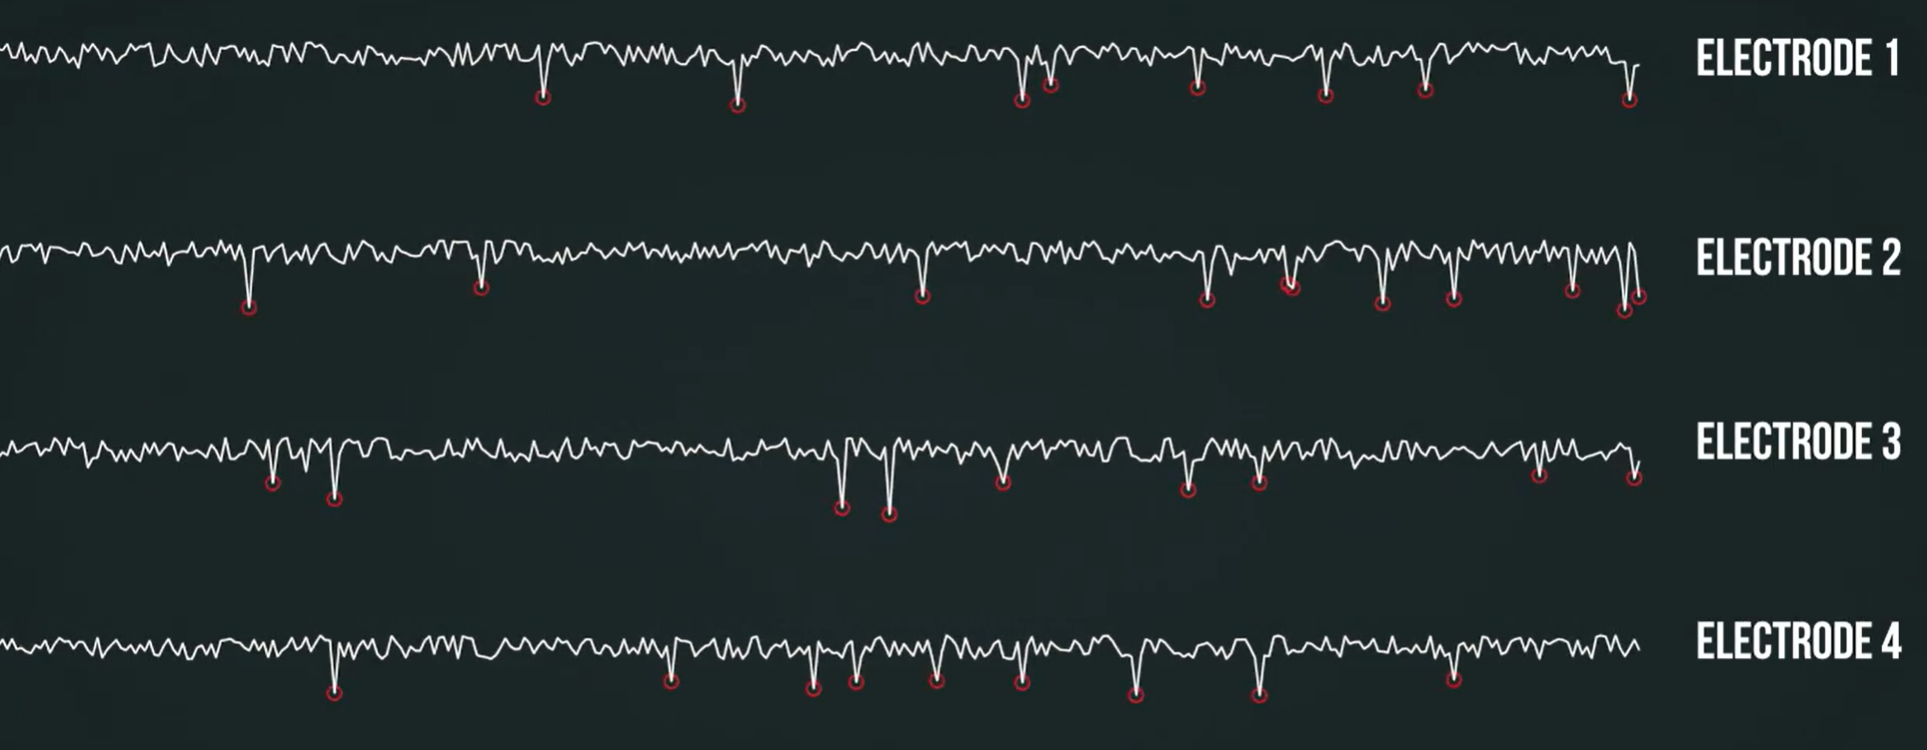
\includegraphics[width=0.9\linewidth]{electrode}
	\end{figure}
\begin{itemize}
	\item Spike train inference is relatively straightforward when high-quality electrical signals are directly recorded (e.g., via simple thresholding methods)
	\item However, such recordings are often invasive and do not scale well to monitoring large populations of neurons simultaneously
\end{itemize}
\end{frame}


\begin{frame}{Calcium imaging: slow but scalable}
	\begin{figure}
		\centering
		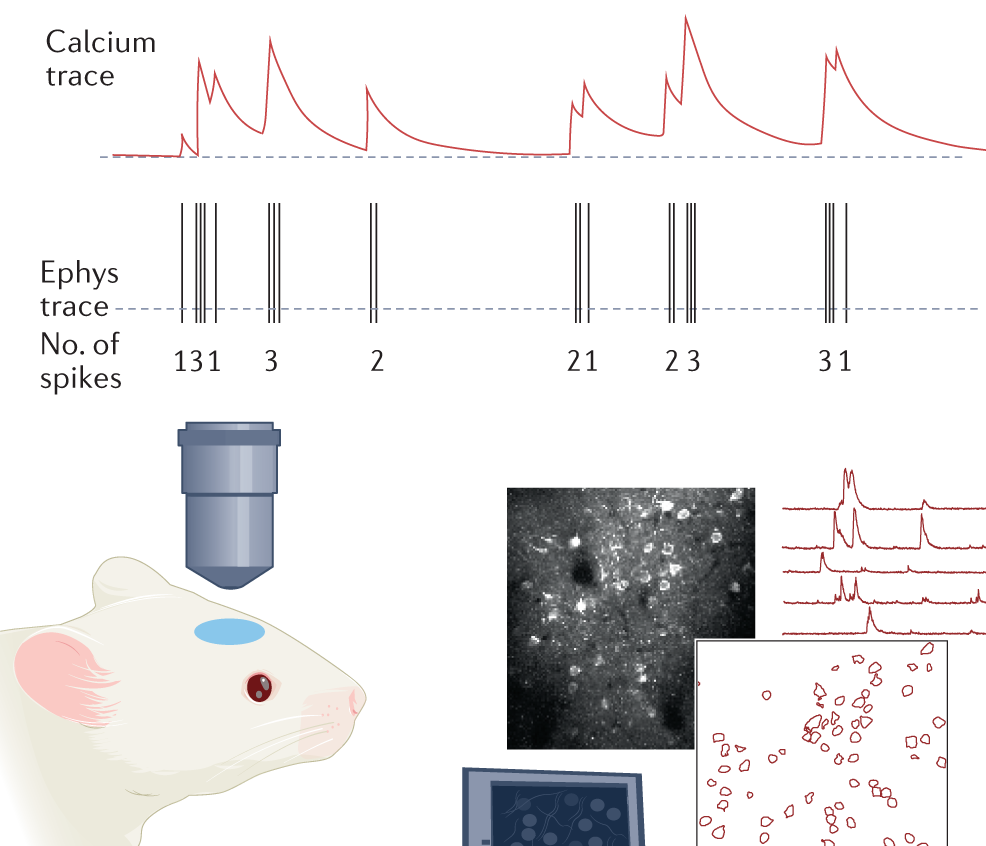
\includegraphics[width=0.7\linewidth]{spikeTrain}
	\end{figure}
	\begin{itemize}
		\item Calcium imaging enables recording from thousands of neurons simultaneously, but its slow dynamics cause signals to overlap
		\item new spikes can occur before previous responses have fully decayed.
	\end{itemize}
\end{frame}

\begin{frame}{Mixed Integer Programming Formulation}
	\begin{figure}
		\centering
		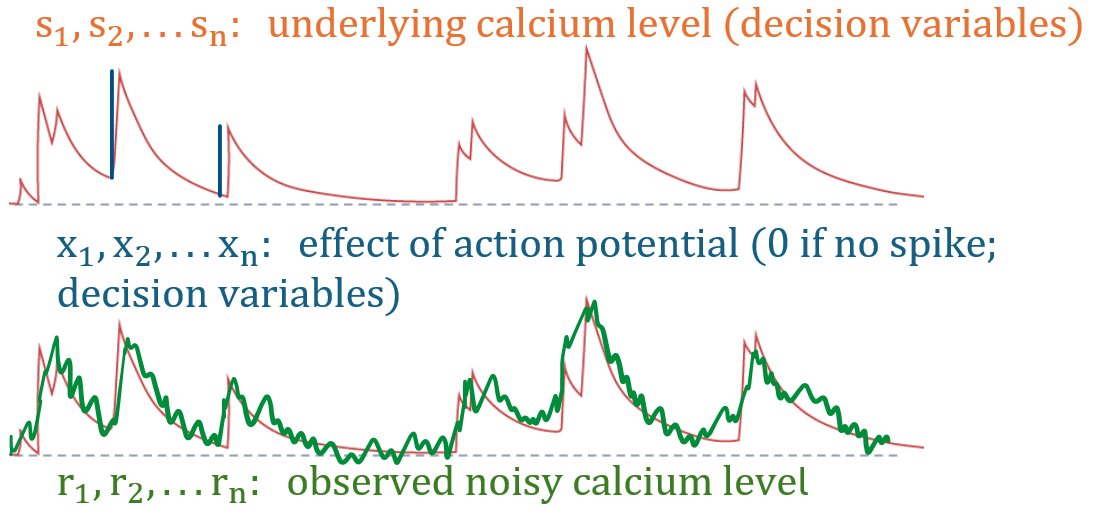
\includegraphics[width=1.05\linewidth]{variables}
	\end{figure}
	To filter out the noise, we solve least squares:
	\begin{equation*}
		\min_{\mathbf{s}} \frac{1}{2}\sum_{i=1}^{n+1}(s_i - r_i)^2
	\end{equation*}
\end{frame}
 
\begin{frame}{Mixed Integer Programming Formulation}
	
	\begin{itemize}
		\item AR(1) model:
		\[
		s_{i+1} = \alpha s_i + x_i
		\]
		\begin{itemize}
			\item Calcium level always decays by $\alpha \in (0,1)$
			\item If $x_i > 0$, there is an effect of an action potential
		\end{itemize}
		
		\item Sparse spikes: add an on-off switch $z_1, \ldots, z_n$ and link it to $x_i$:
		\begin{align*}
			\min_{\mathbf{s}, \mathbf{x}, \mathbf{z}} \quad 
			& \frac{1}{2} \sum_{i=1}^{n+1} (s_i - r_i)^2 + \lambda \sum_{i=1}^n z_i \\
			\text{s.t.} \quad 
			& x_i (1 - z_i) = 0, \quad z_i \in \{0,1\}, \quad i = 1, \ldots, n \\
			& x_i = s_{i+1} - \alpha s_i, \quad i = 1, \ldots, n
		\\& s_1 = 0
		\end{align*}
		
	\end{itemize}
	
\end{frame}
\section{Contributions}
\begin{frame}{Convexification}
The linear dynamic $x_i = s_{i+1} - \alpha s_i$ allows us to project out  $s_i$:
\begin{align*}
	\min_{\mathbf{x}, \mathbf{z}} \quad & \mathbf{x}^\top \mathbf{Q} \mathbf{x} + \mathbf{a}^\top \mathbf{x} + \lambda \sum_{i=1}^n z_i \\
	\text{s.t.} \quad 
	& \mathbf{x} \circ (\mathbf{e} - \mathbf{z}) = 0 
	\quad
 \mathbf{z} \in \{0, 1\}^n,
\end{align*}
where $\mathbf{Q}$ is symmetric and 
$q_{ij} = u_i v_j$, for $i \le j$, where
\begin{align*}
	u_i := \alpha^{n-i}, \quad
	v_i := \frac{\alpha^{2(n-i+1)} - 1}{2\alpha^{n-i}(\alpha^2 - 1)}, 
\end{align*}
\begin{equation*}
	a_i := -\sum_{t=i+1}^{n+1} \alpha^{t-(i+1)} r_t.
\end{equation*}



 
\end{frame}

\section{Model}
\begin{frame}{Convexification}
epigraph formulation:
\begin{align*}
	\min_{\mathbf{x}, \mathbf{z}, \tau} \quad & \tau + \mathbf{a}^\top \mathbf{x} + \lambda \sum_{i=1}^n z_i \\
	\text{s.t.} \quad 
	& (\mathbf{x}, \mathbf{z}, \tau) \in X_Q,
\end{align*}
where
\begin{align*}
	X_Q := \{& (\mathbf{x}, \mathbf{z}, \tau) \in \mathbb{R}^n \times \{0, 1\}^n \times \mathbb{R}_+ :
	\\  &\tau \ge \mathbf{x}^\top \mathbf{Q} \mathbf{x}, \ x_i(1 - z_i) = 0,  i \in [n] \}
\end{align*}
\end{frame}
%
%
\begin{frame}{Convexification}

\begin{equation*}
	\text{cl conv}(X_Q) = C \cap P,   
\end{equation*}
where
\begin{itemize}
	\item 
	$C$ do not restrict   $\mathbf{z}$:
	\begin{align*}
		C :=
		\{& (\mathbf{x}, \mathbf{z}, \tau) \in \mathbb{R}^{2n+1} : \exists \mathbf{W} \in \mathbb{R}^{n \times n}, \mathbf{w} \in \mathbb{R}_+^{(n+1)(n+2)/2} \text{ such that }\\& \begin{bmatrix} \mathbf{W} & \mathbf{x} \\ \mathbf{x}^\top & \tau \end{bmatrix} \succeq 0 \},
	\end{align*}
	
	\item $P$ is a polytope that restricts $\mathbf{z}$ whose corners are integral in $\mathbf{z}$. 
\end{itemize}


 

\end{frame}


%
\begin{frame}{Convexification}
	\begin{itemize}
\item Therefore, the solution of the convex relaxation
 
\begin{align*}
	\min_{\mathbf{x}, \mathbf{z}, \tau} \quad & \tau + \mathbf{a}^\top \mathbf{x} + \lambda \sum_{i=1}^n z_i \\
	\text{s.t.} \quad 
	& (\mathbf{x}, \mathbf{z}, \tau) \in \text{cl conv}(X_Q),
\end{align*}
is feasible for the original problem. 
\item 
This relaxation can be reformulated into shortest path problem for DAG with arc cost which can be solved in $O(n^2)$:
$$
\ell_{ij} = 
\begin{cases} 
	0, & i = 0, \ 1 \le j \le n + 1 \\ 
	\lambda - \dfrac{(1 - \alpha^2) \left( a_i - \alpha^{j-i} a_j \right)^2}{2\left(1 - \alpha^{2(j-i)}\right)}, & 1 \le i < j \le n \\ 
	\lambda - \dfrac{(1 - \alpha^2)a_i^2}{2\left(1 - \alpha^{2(n-i+1)}\right)}, & 1 \le i \le n, \ j = n + 1.
\end{cases}
$$
 \end{itemize}
	\end{frame}
	%
	
 
	
	
	\begin{frame}{The AR(1) paramter $\alpha$}
\begin{itemize}
	\item  $\bar{r} = \frac{1}{n} \sum_{t=1}^n r_t$
	\item   empirical autocovariance at lag $\tau$ is estimated as:
	$$
	\hat{C}_r(\tau) = \frac{1}{N-\tau} \sum_{t=1}^{N-\tau} (r_t - \bar{r})(r_{t+\tau} - \bar{r}).
	$$
	\item Assuming the underlying spiking signal $\mathbf{x}$ originates from a homogeneous Poisson process, and AR(1), we have $C_r(\tau) = \alpha C_r(\tau - 1)$, which yields an estimator:
			$$
	\hat{\alpha} = \frac{\hat{C}_r(2)}{\hat{C}_r(1)}.
	$$
\end{itemize}
\end{frame}

\begin{frame}{Observational noise $\sigma^2$}
 
 
\begin{itemize}
	\item Calcium dynamics are smooth and slow, and therefore primarily concentrated in low-frequency components.
	\item Random jitter from the microscope sensor is distributed uniformly across all frequencies.
	\item Therefore, $\sigma^2$ is estimated by isolating the high-frequency components and computing their variance.
\end{itemize}


\end{frame}

 

\begin{frame}{Sparsity parameter $\lambda$}
	\begin{itemize}
		\item We select $\lambda$ such that the residual sum of squares satisfies
		\begin{equation*}
			\sum_{i=1}^{n} (s_i - r_i)^2 \approx n \sigma^2
		\end{equation*}
		\item For a given $\lambda$, we solve the optimization problem and compute the resulting mean squared error (MSE).
		\item We then compare the MSE to $n \hat{\sigma}^2$ and use a bisection search over $\lambda$ until the target value is reached.
	\end{itemize}
\end{frame}


 

\begin{frame}{Dataset and Comparison}
	\begin{itemize}
		\item 25 real datasets spanning different species (mouse, zebrafish), brain regions, and calcium indicators.
		\item Comparison with a dynamic programming algorithm developed by statisticians (\textit{Jewell and Witten, 2018}).
		\item Precision: TP / (TP + FP)
		\item Recall: TP / (TP + FN)
		\item F1 score: harmonic mean of precision and recall
	\end{itemize}


	\end{frame}

%
%

\bibliographystyle{apalike}
\bibliography{reference}
\end{document}